
%
%%%%%%%%%%%%%%%%%%
%                %
% Introduction   %
%                %
%%%%%%%%%%%%%%%%%%
%
% Brief abstract: introduction to the rest of the work
%
% Completion (1-10): 10
% Missing: Methodology is missing. 
% Proofreading: 7/10/21
% Proofreading: 21/10/21 (integrated reviews) 2x [!]
%
\chapter{Introduction}
\label{cp:intro}

\begin{chapquote}{\cite{wang2017curvature}}
  ``Fixed-wing[s] [...] tend to be more stable in the air in the face of both piloting and technical errors as they have natural gliding capabilities even without power, and they are able to travel longer distances on less power.''
\end{chapquote}

\vspace*{1em}

\lettrine{M}{obile robots} have the ability to move~\citep{corke2017robotics} and eventually sense and interact with the surrounding environment. They combine and interpret data from multiple components~\citep{mei2006deployment}, using various algorithms for perception and planning\findex{perception algorithms}. For instance, with a motion planning\findex{motion planning} algorithm, a mobile robot converts a human-level plan with sensing into machine-level motion primitives~\citep{lavalle2006planning}\findex{motion primitives}. There are numerous planning algorithms applied to a variety of robots. Some, including motion planning and obstacle avoidance, are mature enough to be transferred onto real-world use cases~\citep{siciliano2016bspringer}. These algorithms often run on energy-demanding heterogeneous computing hardware\findex{heterogeneous computing hardware} onboard the mobile robots. They share computational capabilities with other algorithms, enabling various autonomous features. In this context, energy consumption is a crucial aspect~\citep{jaiem2016step}. Most mobile robots have strict battery limitations, affecting the computing hardware and influencing the autonomous features\findex{autonomy}, in turn, expected to increase in the foreseeable future~\citep{fisher2013verifying}.

While there are planning approaches that are well covered, others have received little attention from the research community. Planning-scheduling\findex{planning}\findex{scheduling} energy awareness is one of such underrepresented approaches in the robotics research literature~\citep{sudhakar2020balancing,lahijanian2018resource,ondruska2015scheduled,brateman2006energy}. Here, by planning-scheduling energy awareness, we mean the derivation of an energy-aware path with a power-saving scheduling policy for the computing hardware. Past studies cover extensively one of these topics, but their interactions are largely unexplored~\citep{brateman2006energy}. Some generate an energy-optimized path, but the computations\findex{computations} energy--the energy required by the power demanding tasks running on the computing hardware--might equal the motion in some instances of low-energy mobile robots~\citep{sudhakar2020balancing}. Due to the recent advancements in the computational capabilities of heterogeneous computing hardware, such as the introduction of powerful portable GPUs\findex{GPU}~\citep{rizvi2017general}, the use of computations is then further on the rise~\citep{abramov2012real,satria2016real,jaramillo2019visual}. Others provide a power-saving scheduling policy, yet, moving a mobile robot requires considerable energy expenditure over mere computations~\citep{mei2004energy,mei2005case}.

We trade both planning-scheduling altogether and under strict energy constraints. Within motion planning itself, by focusing on a specific category. In autonomous scenarios, it is often required to explore every location in space~\citep{cao1988region,choset2000exact,arkin2001optimal,arkin2005optimal}. A problem solved by coverage planning~\citep{choset2001coverage,galceran2013survey}\findex{coverage path planning}, and so, we show the interactions between planning-scheduling on a coverage planning algorithm, covering a space scheduling high-level task for, e.g., perception, in an elemental region\findex{elemental region}. As a mobile robotics platform, we evaluate the approach with aerial mobile robots in simulations and empirical trials. Although sharing with the broader class of mobile robots stringent battery limitations, they have additional impediments. A conventional setup would require landing to replace or recharge the battery. {\itshape Aerial robots are an ideal instance of energy-constrained systems, benefitting the simultaneous planning-scheduling energy awareness}. We will see that we can back such a statement with observations of actual flights failure reductions later with this work in \fref{cp:res}{Chapter}.

\begin{figure}[t!]
  \centering
  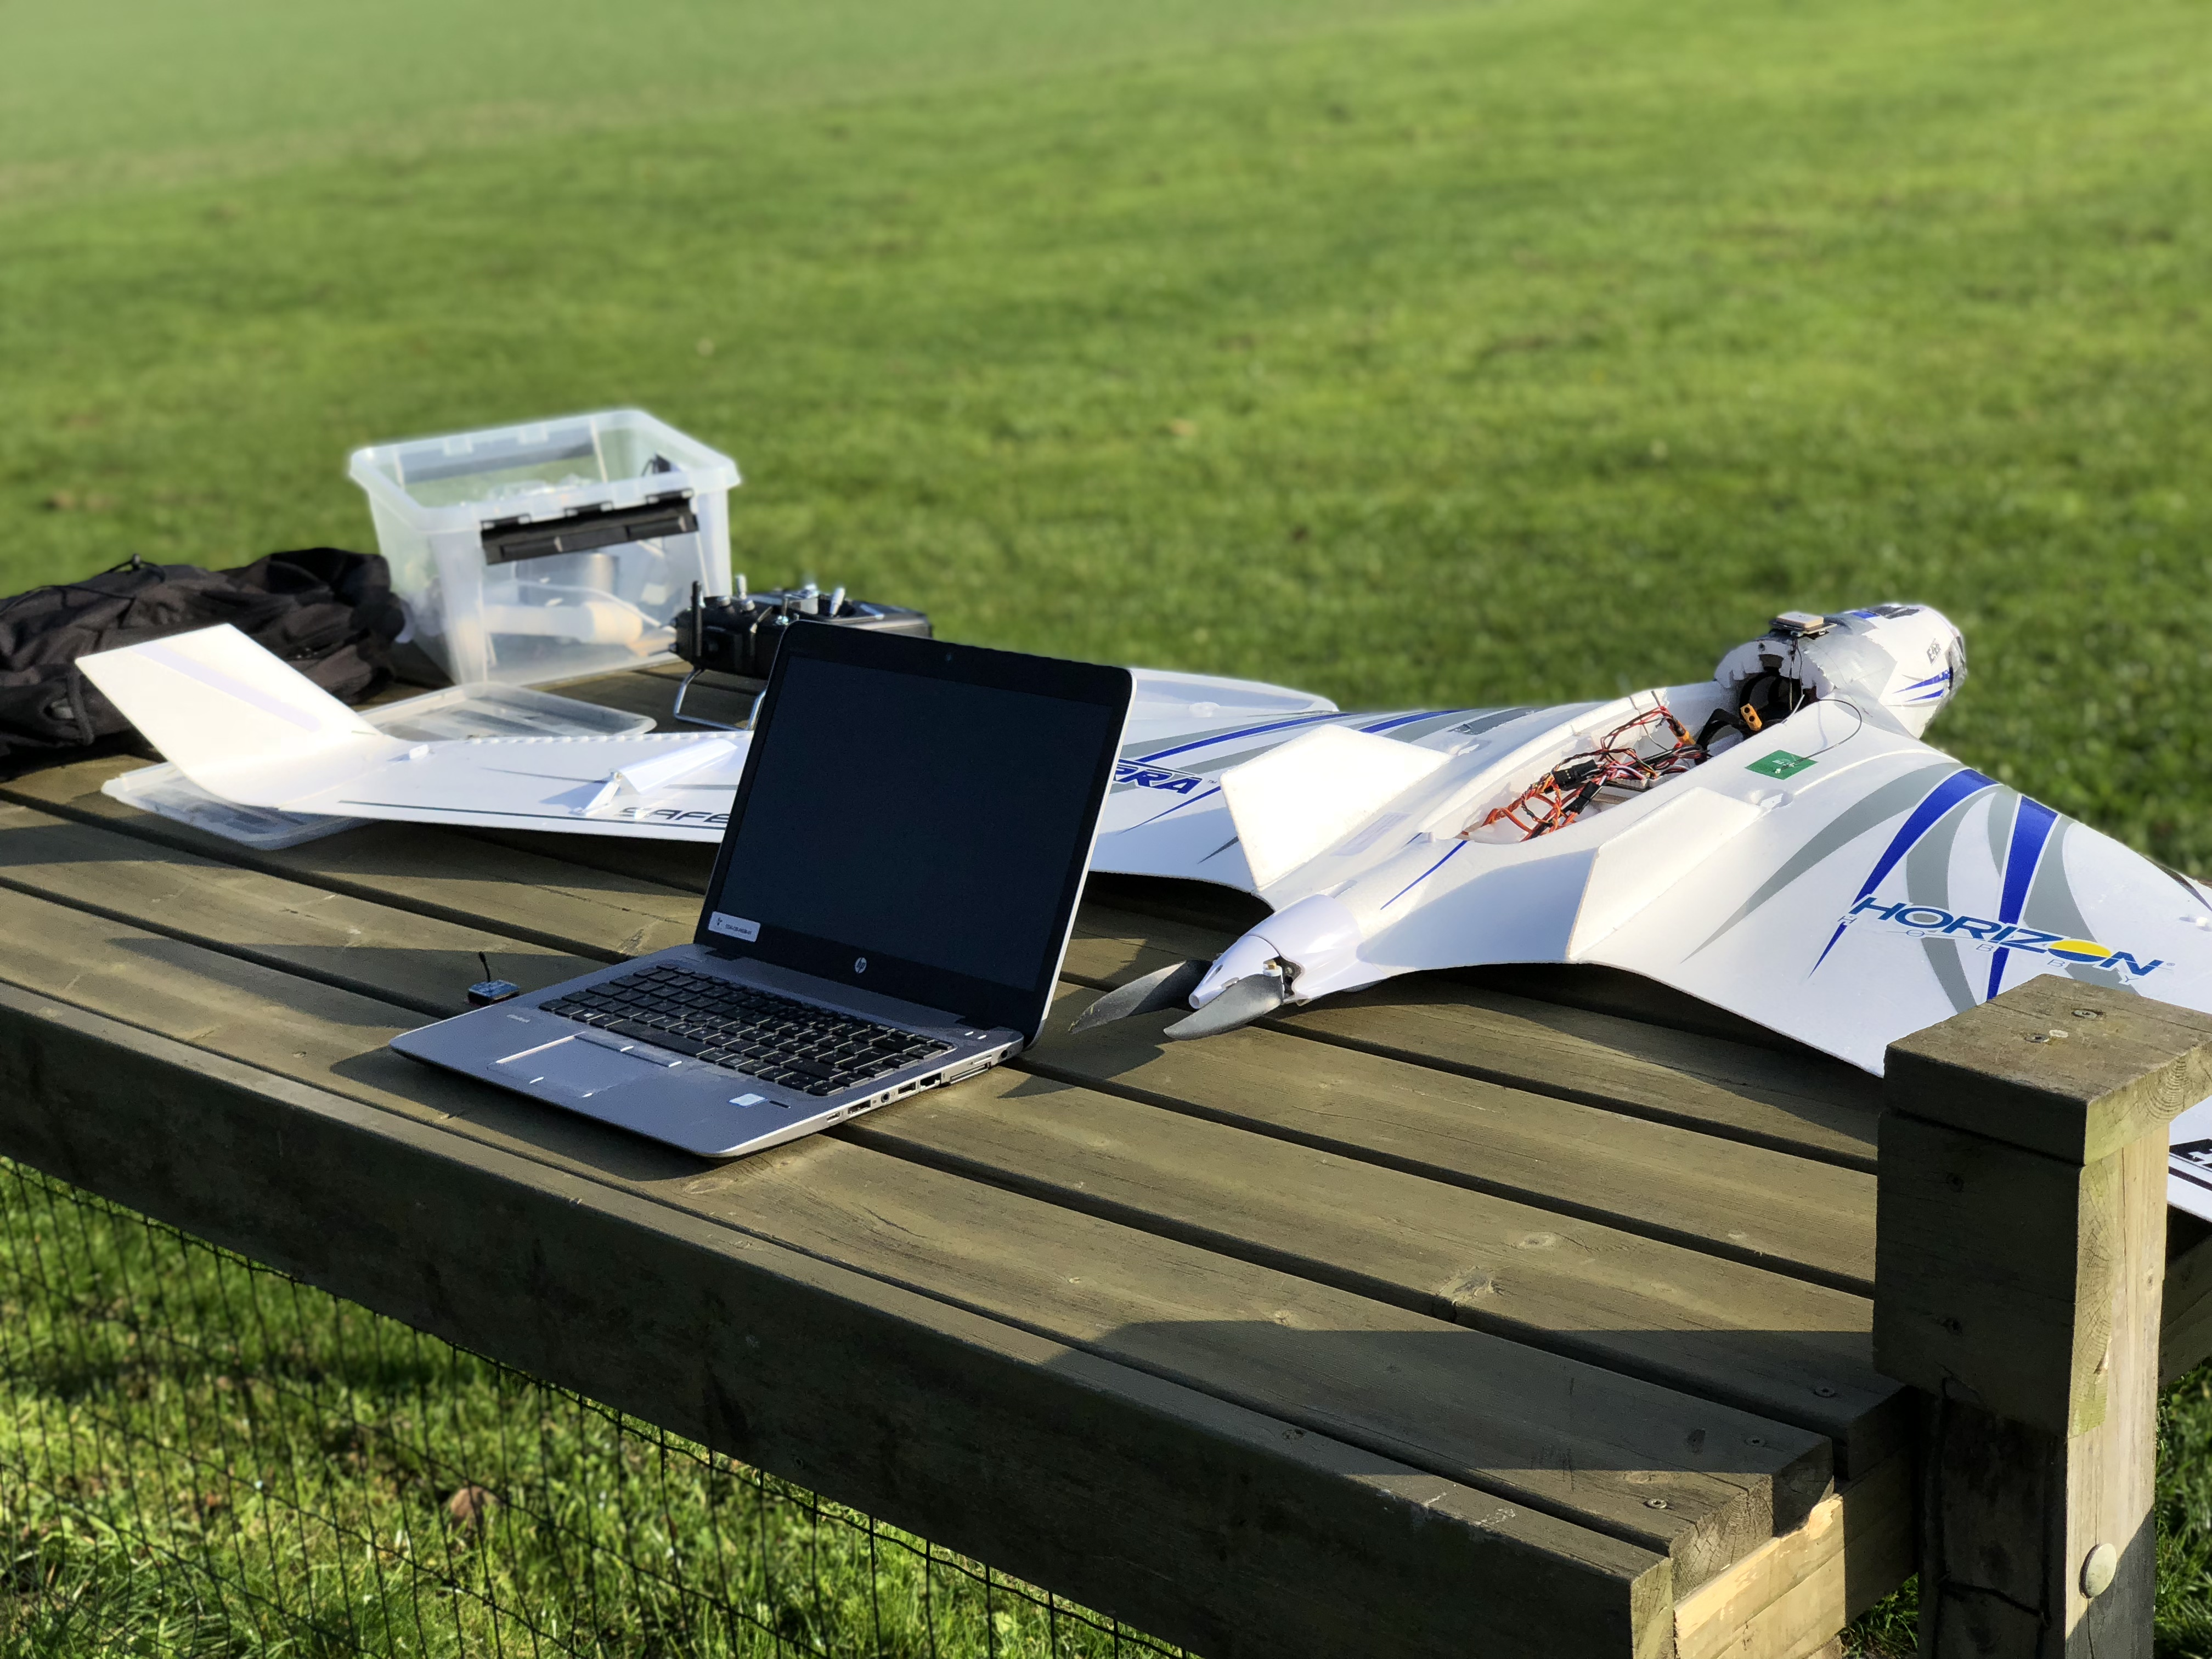
\includegraphics[width=.7\textwidth]{pictures/photo}
  \caption[Opterra fixed-wing aerial robot for the precision agriculture use case]{Opterra fixed-wing aerial robot for the precision agriculture use case {\scriptsize(photo credit: Amit Ferencz Appel)}.}
  \label{fig:opterra}
\end{figure}
There are numerous autonomous use cases involving aerial robots, such as precision agriculture, search and rescue\findex{search and rescue}, payload delivery\findex{payload delivery}, transportation\findex{transportation}, and many others. Here, we focus on a precision agriculture use case of an autonomous aerial robot flying over an agricultural field with little human input. Precision agriculture\findex{precision agriculture} is indeed often put into practice~\citep{hajjaj2014review} with ground mobile robots used for harvesting~\citep{qingchun2012study,dong2011development, de2011design, aljanobi2010setup, li2008analysis, edan2000robotic}, and aerial robots for preventing damage and ensuring better crop quality~\citep{puri2017agriculture, daponte2019review}. We investigate different physical aerial robotics platforms in this work but derive most results with the Opterra fixed-wing\findex{Opterra fixed-wing aerial robot}~\citep{opterra} adapted for precision agriculture. The aerial robot is in \fref{fig:opterra}{Figure}.

The scope of this chapter is to introduce and motivate the planning-scheduling energy awareness for aerial robots. To this end, \fref{sec:history}{Section} investigates the evolution of aerial robots, and \fref{sec:aerial-robo-types}{Section} classifies the modern aerial robotics literature w.r.t. this work. \fref{sec:motivation}{Section} provides further motivation, objective, and methodology, and \fref{sec:outline}{Section} outlines the approach. \fref{sec:applics}{Sections}\fref{sec:contribs}{--\hspace*{-.8ex}} contain discussions of possible application and overall contribution. Finally, \fref{sec:structure}{Section} structures the remaining chapters.

% [!] Unnecessary text as it is already in the last section! Erased.
%This chapter connects to the remainder of this work as follows. Here we introduce and motivate energy-aware coverage planning and scheduling for autonomous aerial robots. We formalize the problems in \fref{cp:pb}{Chapter}, and discuss previous relevant approaches in the literature in \fref{cp:soa}{Chapter}. We derive an energy model to predict future energy consumption in \fref{cp:model}{Chapter} and an optimal configuration of the path and computations using data-driven control\findex{data-driven control} and other modern optimal control techniques in \fref{cp:dyn}{Chapter}. In the same chapter, we provide some details for guidance, which physically moves the robot. We discuss the experimental setup and results in \fref{cp:res}{Chapter}.


%%%%%%%%%%%%%%%%%%%%%%%%%%%%%%%%%%%%%%%%%%%
\section{From UAVs to Modern Aerial Robots}
\label{sec:history}

Modern aerial robots are a valuable tool in robotic research and aerospace and have different names in the literature, including unmanned aerial vehicles\findex{unmanned aerial vehicles} (\Gls{acr:uav}s)\footnote{The term unmanned is sometimes replaced by uninhabited.}, unmanned aerial systems\findex{unmanned aerial systems} (\Gls{acr:uas}s)\footnote{UAS often denotes the entire infrastructure of unmanned flight in the aerospace jargon.}, flying robots, or drones. Usually, UAVs and UASs indicate that these systems are semi-autonomous or operated from the ground, whereas aerial or flying robots have advanced levels of autonomy~\citep{siciliano2016springer}. Nevertheless, all these systems have basic autonomous features such as position holding implemented with, e.g., the global navigation satellite system\findex{global navigation satellite system} (\Gls{acr:gnss}), altitude holding with a barometer\findex{barometer}, and leveling with the inertial measurement unit\findex{inertial measurement unit} (\Gls{acr:imu}).

\begin{figure}[t]
  \centering
  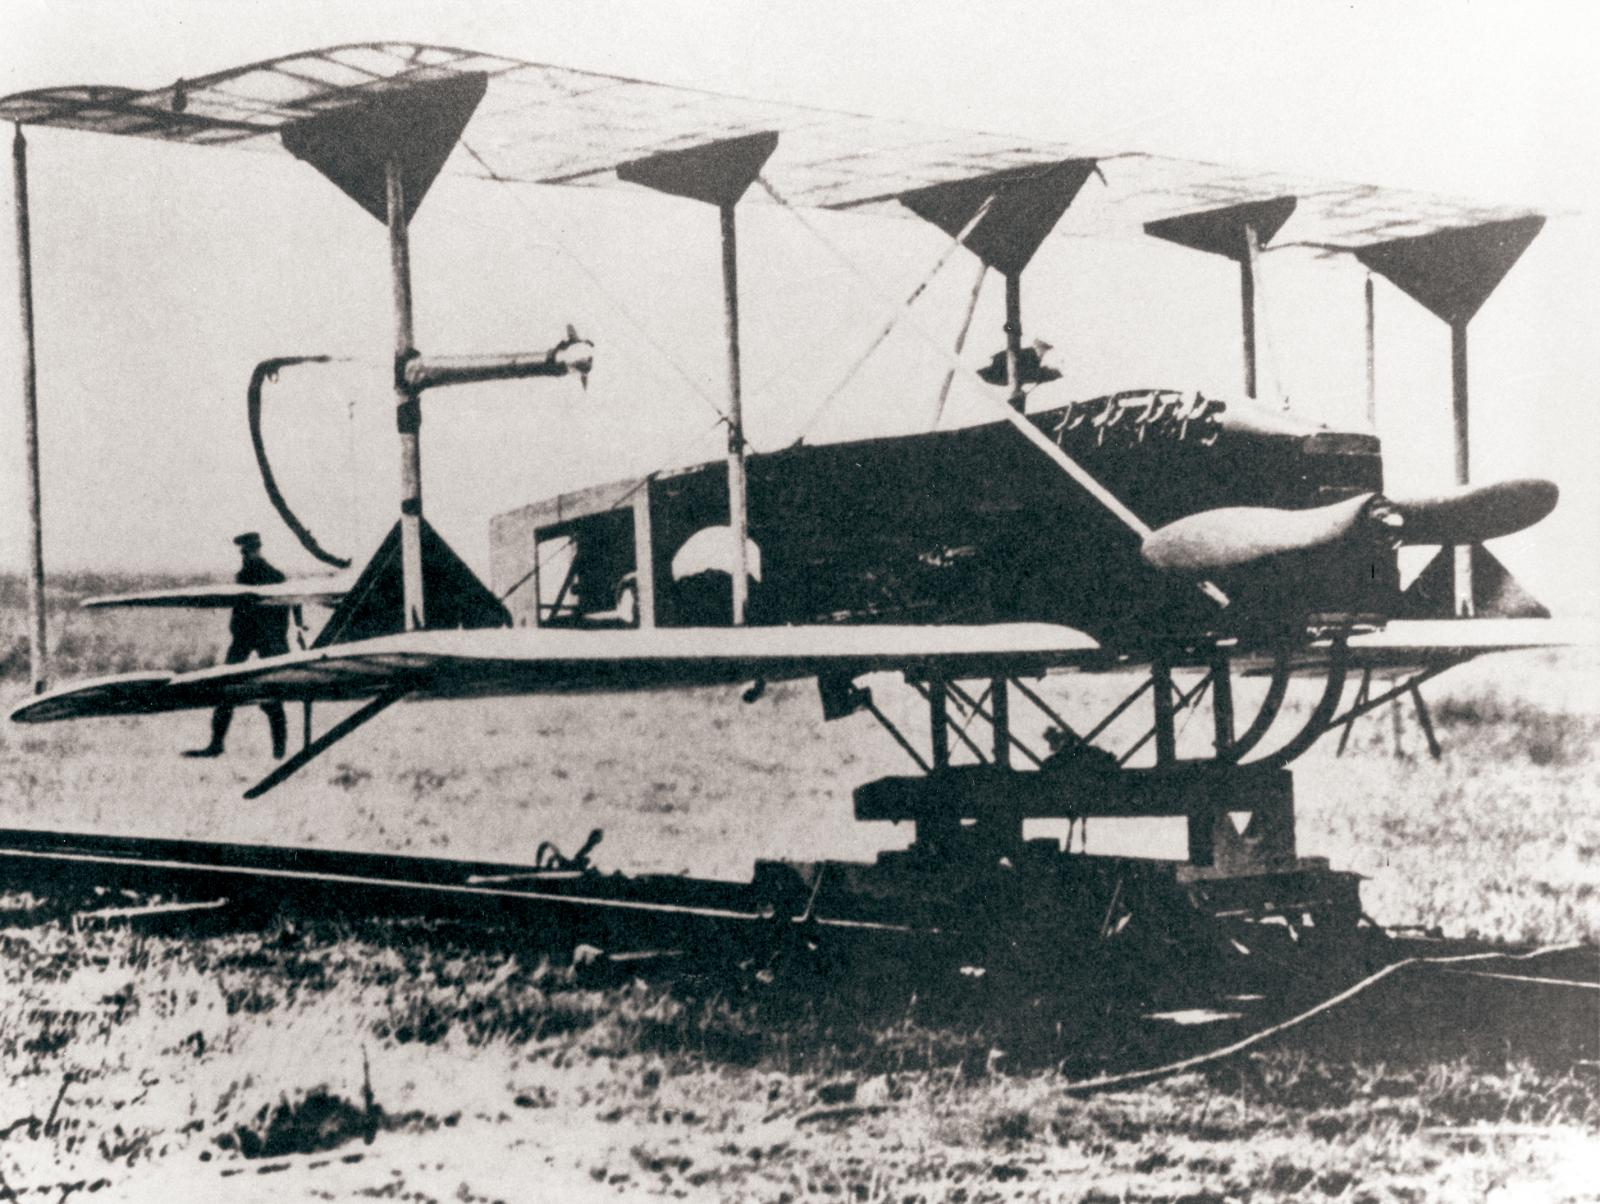
\includegraphics[width=.7\textwidth]{pictures/HA-NH-JA-19_1}
  \caption[Hewitt-Sperry Automatic Airplane, the first unmanned flying machine]{The Hewitt-Sperry Automatic Airplane, denominated ``flying bomb'' and developed during WWI, represents the first instance of a \Gls{acr:uav} {\scriptsize(photo credit: United States Naval Institute)}.}   
  \label{fig:hewitt-sperry}
\end{figure}
Unmanned (or uninhabited) flight has more than a century of developments~\citep{siciliano2016springer}. The origin of the field, which deals with the design and development of aerial robots, dates back to the first guided missiles. Hewitt-Sperry Automatic Airplane\findex{Hewitt-Sperry automatic airplane} in \fref{fig:hewitt-sperry}{Figure}, also denominated ``flying bomb'' and deployed in 1917 during World War~I\findex{World War I}~(WWI)~\citep{keane2013brief,valavanis2015handbook}, is often referred to as the first unmanned flying machine. Developed 14 years after the first heavier-than-air flight in history--demonstrated on December 17, 1903, with the Wright Flyer I by Wilbur and Orville Wright\findex{Wright brother} (or the Wright brothers)--it used a gyroscope\findex{gyroscope}, invented shortly before by Elmer Sperry~\citep{keane2013brief}, like modern aerial robots. The device was mechanically connected to the control surfaces, successfully implementing a control feedback loop~\citep{siciliano2016springer}.

In their early days, these first flying machines were referred to as remotely piloted vehicles\findex{remotely piloted vehicles} (\Gls{acr:rpv}s)~\citep{anderson2005introduction}. Many instances from WWI served military purposes. In the 1950s, the United States used an RPV, the Ryan Firebee\findex{Ryan Firebee}, for reconnaissance in Vietnam, and Israel was the first to use an RPV in a combat situation~\citep{anderson2005introduction}. Other instances include the V-1 flying bomb~\findex{V-1 flying bomb} from 1944 (deployed by the unified armed forces of nazi Germany) and the Lockheed D-21~\findex{Lockheed D-21} from 1962 (deployed by the United States Air Force). The introduction of the global positioning system\findex{global positioning system} (\Gls{acr:gps}) at the end of 1970 soared recent developments with applications such as surveillance. Integration with cameras and other sensors grounded further applications~\citep{siciliano2016springer}, introducing modern aerial robots.

Recent developments include many civilian applications~\citep{gonzalez2017unmanned}. Aerial robots are used increasingly in remote sensing\findex{remote sensing}~\citep{colomina2014unmanned,noor2018remote,tang2015drone,milas2018drones}, surveillance\findex{surveillance}~\citep{acevedo2014one,ramasamy2017heuristic,basilico2015deploying,paucar2018use,burkle2009collaborating}, meteorology\findex{meteorology}~\citep{renzaglia2016monitoring,schuyler2019using}, search and rescue\findex{search and rescue}~\citep{hayat2017multi,pensieri2020drones,karaca2018potential,cui2015drones,seguin2018unmanned}, precision agriculture~\citep{popovic2017online,sa2018weednet,lottes2017uav,daponte2019review,puri2017agriculture}, transportation, and payload delivery\findex{payload delivery}~\citep{kellermann2020drones}. The former four categories fall into reconnaissance, surveillance, and target acquisition\findex{reconnaissance, surveillance, and target acquisition} (\Gls{acr:rsta}) and do not require advanced autonomy; precision agriculture, transportation, and payload delivery utilize a certain extent of computational intelligence~\citep{siciliano2016springer}. They handle unexplored terrain with little interaction, contrary to the past human-operated UAVs~\citep{siciliano2016springer}. Instances autonomously adapt and possibly interact in a wide variety of environmental conditions.

\begin{figure}[t]
  \centering
  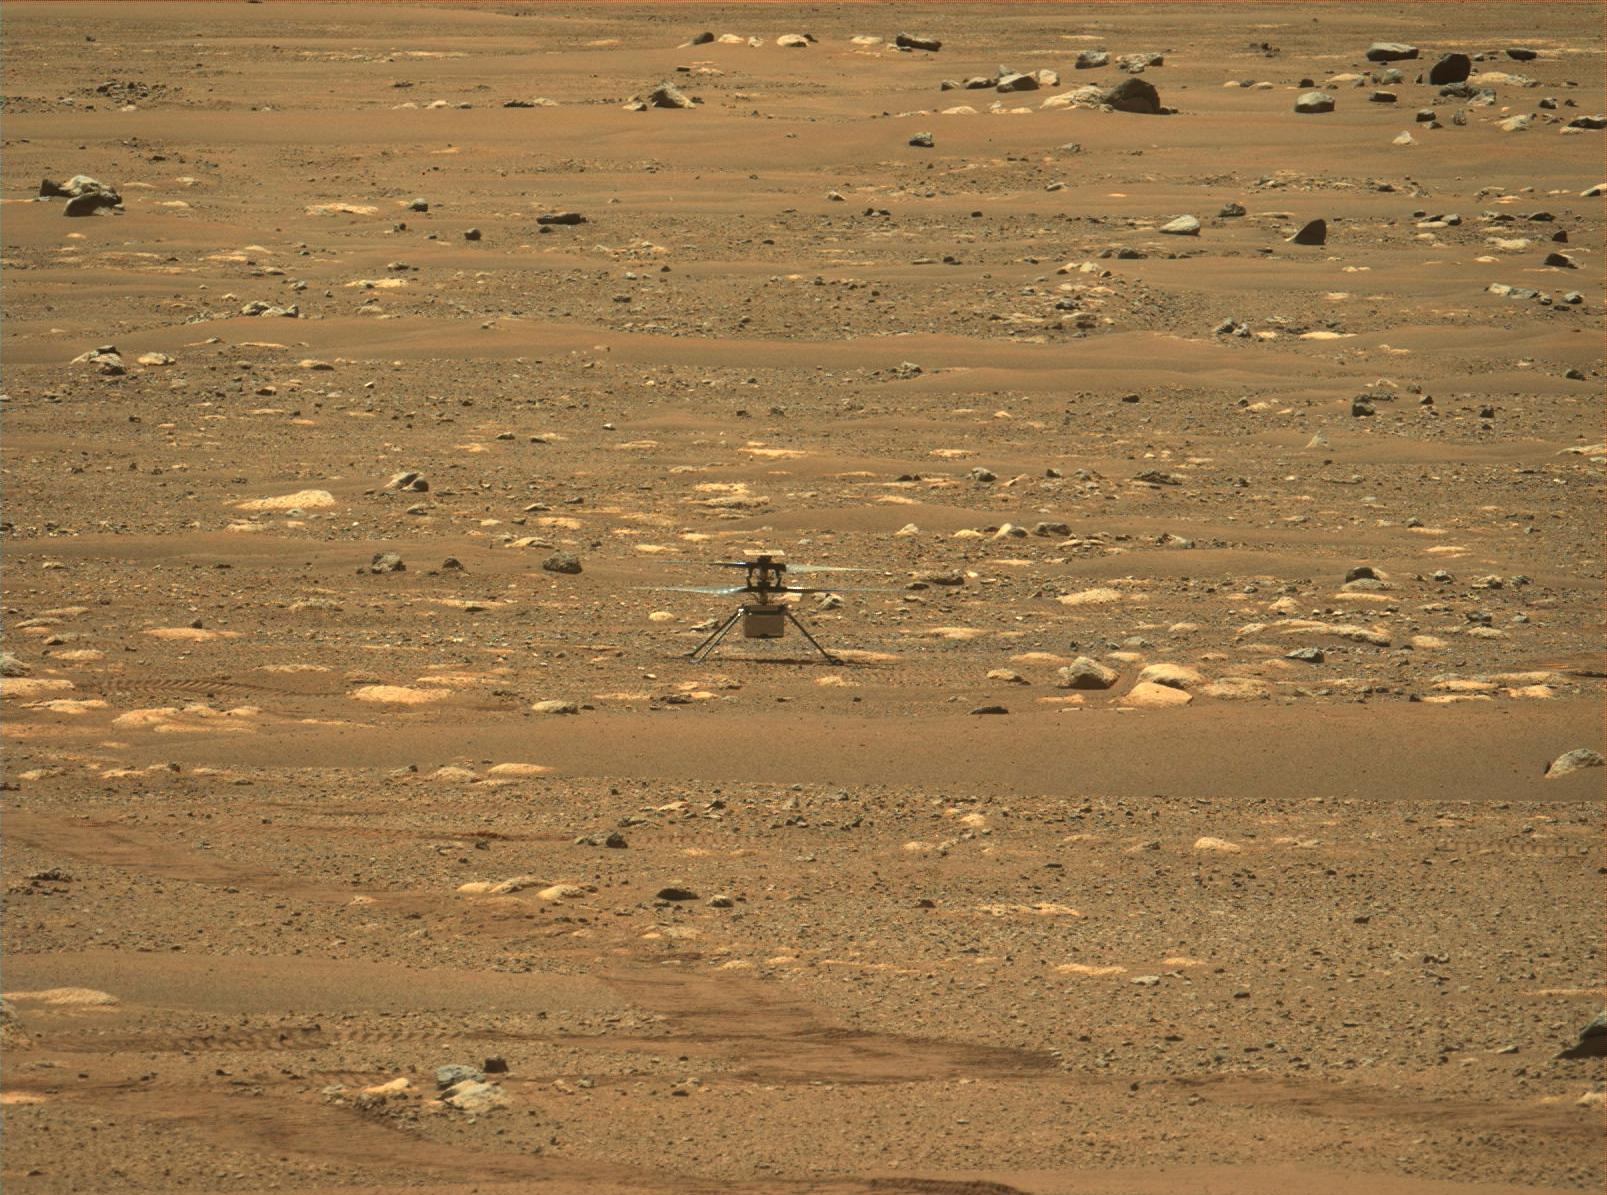
\includegraphics[width=.7\textwidth]{pictures/jpegPIA24550}
  \caption[NASA's Ingenuity Mars Helicopter]{NASA's Ingenuity Mars Helicopter. A rotary-wing coaxial aerial robot, achieving the first powered, controlled flight on another planet on April 19, 2021 {\scriptsize(photo credit: NASA Jet Propulsion Laboratory)}.}   
  \label{fig:ingenuity}
\end{figure}
In summary, aerial robots have a recent past. Some initial experiments came shortly after the first heavier-than-air manned and powered flight. These often served military purposes, whereas modern aerial robots fly in a broad range of civilian applications. Aerial robots are to grow significantly in numerous areas in and out of robotics research ranging from agriculture to planetary exploration. For the latter, \fref{fig:ingenuity}{Figure} shows NASA's Ingenuity Mars Helicopter\findex{Ingenuity Mars Helicopter}\findex{NASA}. A small coaxial aerial robot\findex{coaxial aerial robot}\findex{Mars} in the first powered, controlled flight on another planet on April 19, 2021. Aerial robots for planetary exploration are to be deployed in future explorations endeavors, for instance, to study Saturn's moon Titan~\citep{voosen2019nasa}\findex{Saturn}\findex{Titan}.


%%%%%%%%%%%%%%%%%%%%%%%%%%%%%%%%%%%%%%%%%
\section{Common Classes of Aerial Robots}
\label{sec:aerial-robo-types}

There are different types of aerial robots in the robotics literature. We briefly investigate the most studied classes w.r.t. the planning-scheduling energy awareness in this work. The two most generic classes are heavier-\findex{heavier-than-air aerial robots} and lighter-than-air aerial robots. Heavier-than-air compromise fixed- and rotary-wings~\citep{siciliano2016springer}, and some recent contributions in bio-inspired robotics investigate flapping-wings aerial robots~\citep{floreano2015science}\findex{flapping-wings}.


Rotary-wing aerial robots\findex{rotary-wings} are highly maneuverable and suited for stationary vertical flight or hovering\findex{hovering}~\citep{siciliano2016springer}. They compromise multirotors\findex{multirotors} (equipped with multiple rotors such as quadrotors\findex{quadrotors} or quadcopters\findex{quadcopters}, hexacopters\findex{hexacopters}, and octocopters\findex{octocopters}), conventional helicopters\findex{helicopters} (with one main and one tail rotor), and coaxes\findex{coax} (with counter-rotating coaxial rotors)~\citep{corke2017robotics}. Examples of quadrotors are DJI Mavic Mini in \sref{lab:mavic}{} and DJI Phantom 4 in \sref{lab:phantom}{} in \fref{fig:robots-vs-power}{Figure}. DJI Agras T16 in \sref{lab:agras}{} and DJI Matrice 600 in \sref{lab:matrice}{} are hexacopters.

Fixed-wing aerial robots\findex{fixed-wings} share the same motion principle with an aircraft where wings provide the lift, control surfaces maneuvering, and propellers the forward thrust~\citep{corke2017robotics}. An example constitutes the Opterra adapted for precision agriculture in \fref{fig:opterra}{Figure}, Cumulus in \sref{lab:cumulus}{}, Ebee in \sref{lab:ebee}{}, and Penguin BE in \sref{lab:penguin}{}~\citep{haugen2016monitoring} in \fref{fig:robots-vs-power}{Figure}. Examples of flapping-wings are DelFly II in \sref{lab:delfly}{}~\citep{percin2012flow,groen2010improving,clercq2009aerodynamic} and Nano-Hummingbird in \sref{lab:nano}{}. Instances of lighter-than-air aerial robotss\findex{lighter-than-air aerial robots} are blimps\findex{blimps} (or non-rigid airships). They usually rely on gas, e.g., helium\findex{helium} enclosed in a protected envelope~\citep{burri2013design}, to generate the lifting force\findex{lift}~\citep{fui2017recent}. An omnidirectional spherical blimp is in \fref{fig:skye-blimp}{Figure}. Blimps are similar to balloons but provide some maneuverability against controlling merely the altitude~\citep{colombatti2011lighter}.
\begin{figure}[t]
  \centering
  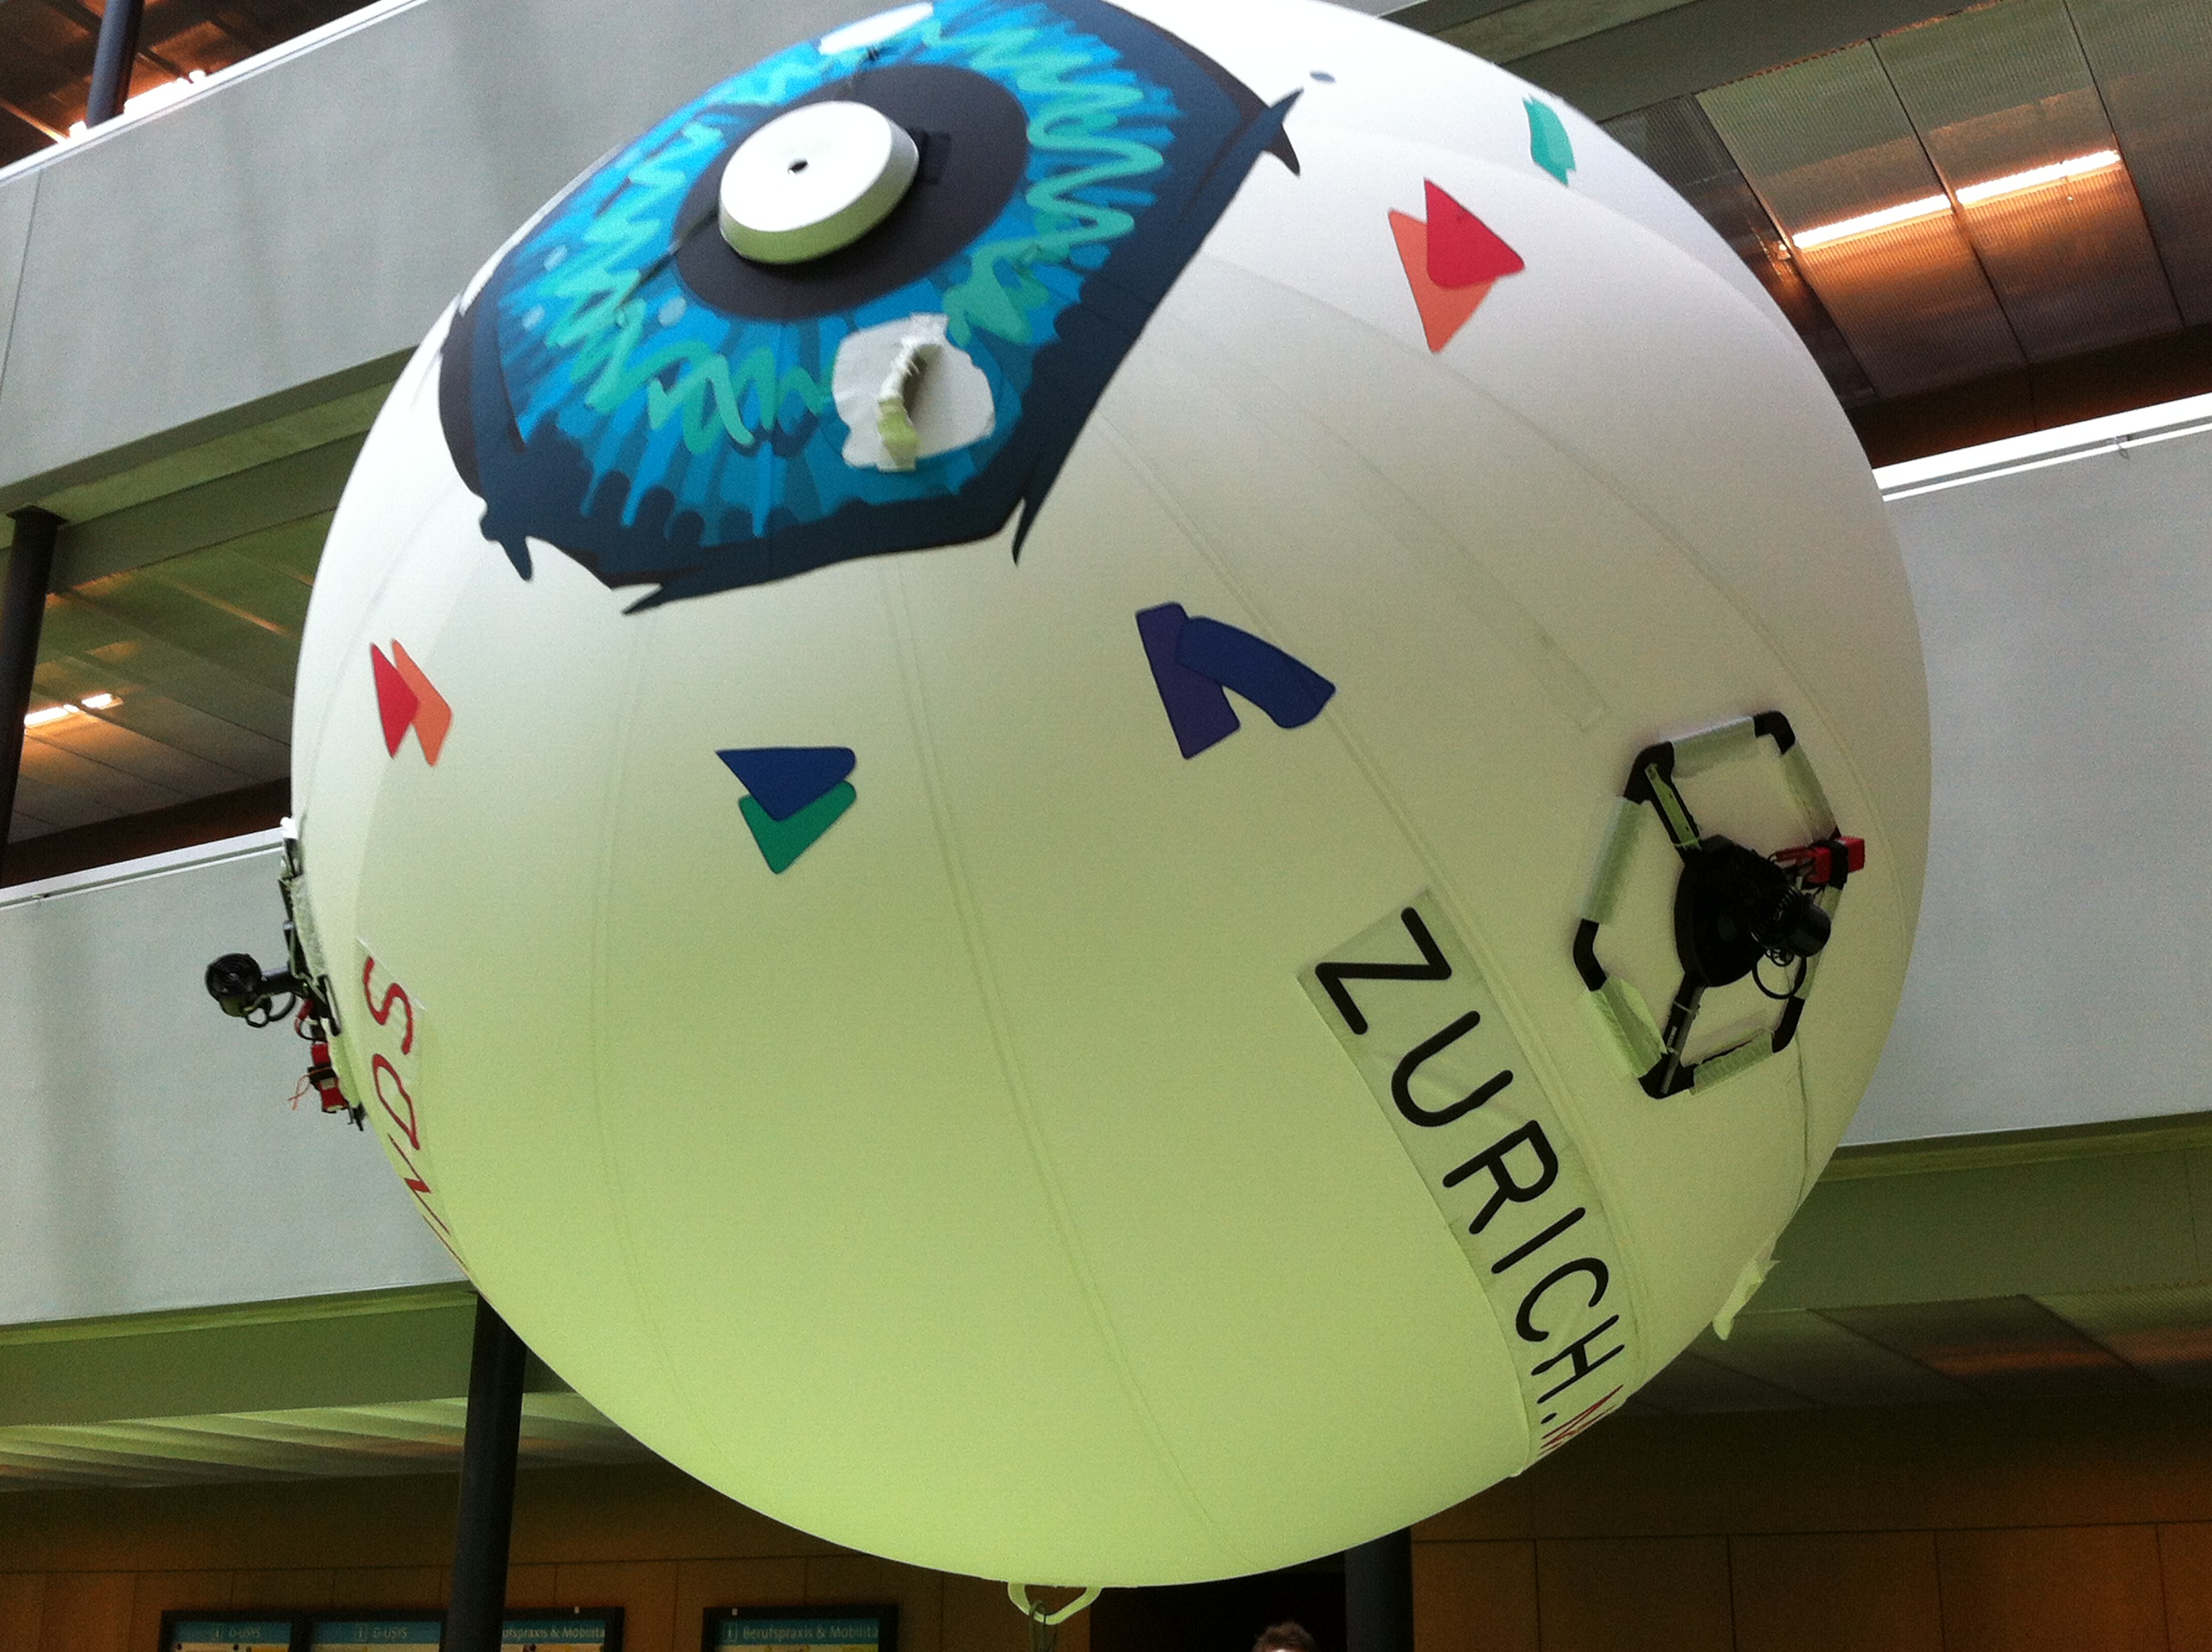
\includegraphics[width=.7\textwidth]{pictures/IMG_2612}
  \caption[Skye, an omnidirectional spherical blimp]{Skye, an omnidirectional spherical blimp developed by ETH Z\"urich for entertainment purposes. It has a camera system and combines the energy-efficient flight of a blimp with the characteristics of a quadrotor {\scriptsize(photo credit: ETH Z\"urich)}.}   
  \label{fig:skye-blimp}
\end{figure}
Other classifications are, e.g., micro aerial vehicles (\Gls{acr:mav}s)\findex{micro aerial vehicles}, vertical take-off and landing (\Gls{acr:vtol}s)\findex{vertical take-off and landing} aerial robots, and others. The former are aerial robots with all dimensions lower than 15 centimeters. The latter fly in a fixed-wing configuration except for taking-off and landing, where they use thrust\findex{thrust} from rotors rather than lift from wings.

\begin{figure}[p!]
  \centering
  \footnotesize\fontfamily{phv}\selectfont
  
\definecolor{cCCD3DA}{RGB}{204,211,218}
\definecolor{cE6E8E9}{RGB}{230,232,233}
\definecolor{c6884A1}{RGB}{104,132,161}
\definecolor{cFFFFFF}{RGB}{255,255,255}


\def \globalscale {1.100000}
\begin{tikzpicture}[y=0.80pt, x=0.80pt, yscale=-\globalscale, xscale=\globalscale, inner sep=0pt, outer sep=0pt]
\path[fill=cCCD3DA,line join=round,line width=0.160pt] (66.7805,413.4660) .. controls (66.7805,413.4660) and (78.2497,419.4630) .. (79.6039,419.5840) .. controls (89.0833,420.4270) and (120.7060,425.6230) .. (132.8490,418.9240) .. controls (132.8490,418.9240) and (147.1650,416.0520) .. (162.4250,406.6130) .. controls (177.6850,397.1740) and (154.6790,353.8840) .. (154.6790,353.8840) .. controls (154.6790,353.8840) and (150.3670,348.0420) .. (140.6380,337.6960) .. controls (120.8650,316.6680) and (96.0032,313.8320) .. (96.0032,313.8320) .. controls (96.0032,313.8320) and (34.4821,288.0000) .. (25.3585,301.5340) .. controls (25.3585,301.5340) and (-20.7738,319.8260) .. (41.4462,396.1850) -- (66.7805,413.4660) -- cycle;

\path[fill=cE6E8E9,line join=round,line width=0.160pt] (142.1740,297.1340) .. controls (142.1740,297.1340) and (148.7360,277.7050) .. (173.0500,271.2740) .. controls (197.3650,264.8420) and (245.9940,267.9790) .. (294.6230,254.2530) .. controls (343.2520,240.5270) and (383.6380,271.2740) .. (383.6380,271.2740) .. controls (383.6380,271.2740) and (421.5680,319.1960) .. (351.0560,362.1000) .. controls (280.5440,405.0040) and (204.1500,362.5510) .. (197.3650,356.6060) .. controls (190.5800,350.6600) and (152.6630,352.7500) .. (144.3720,337.7850) .. controls (136.0820,322.8200) and (136.0140,310.1020) .. (142.1740,297.1340) -- cycle;

\path[fill=c6884A1,line join=round,line width=0.160pt] (169.9270,243.5050) .. controls (169.9270,243.5050) and (176.2790,258.5180) .. (226.4820,251.2460) .. controls (235.3200,249.9660) and (240.0200,249.7140) .. (254.5200,240.2070) .. controls (298.9310,211.0850) and (279.1500,193.9810) .. (285.6770,180.4930) .. controls (291.4950,168.4730) and (299.0130,155.0360) .. (299.0130,155.0360) .. controls (299.0130,155.0360) and (306.9370,126.7230) .. (296.2390,109.5960) .. controls (261.7860,54.4380) and (213.1670,70.7288) .. (213.1670,70.7288) .. controls (213.1670,70.7288) and (183.8340,72.3287) .. (170.9270,88.4355) .. controls (170.9270,88.4355) and (151.0320,100.5190) .. (150.3600,147.3040) .. controls (150.3600,147.3040) and (152.9850,198.8730) .. (155.3740,203.6210) .. controls (157.6800,208.2050) and (169.6860,243.3170) .. (169.9270,243.5050) -- cycle;

\path[fill=foo,line join=round,line width=0.160pt] (126.1400,97.1736) .. controls (126.1400,97.1736) and (153.8360,27.5329) .. (70.0033,24.4741) .. controls (-15.4922,21.3547) and (64.0333,197.2630) .. (126.1400,97.1736) -- cycle;

\path[cm={{1.0,0.0,0.0,1.0,(0,0)}}] (0.0000,0.0000) node[below right] () {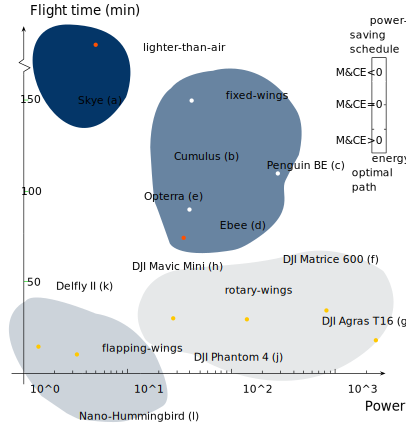
\includegraphics[width=4.95in]{figures/source/plot10}};


\path[fill=foo,line join=round,line width=0.160pt] (376.1380,338.2660) .. controls (377.3320,338.2660) and (378.3000,339.2340) .. (378.3000,340.4280) .. controls (378.3000,341.6220) and (377.3320,342.5900) .. (376.1380,342.5900) .. controls (374.9440,342.5900) and (373.9750,341.6220) .. (373.9750,340.4280) .. controls (373.9750,339.2340) and (374.9440,338.2660) .. (376.1380,338.2660) -- cycle;



\path[fill=foo,line join=round,line width=0.160pt] (326.6650,308.4460) .. controls (327.8590,308.4460) and (328.8270,309.4140) .. (328.8270,310.6080) .. controls (328.8270,311.8020) and (327.8590,312.7700) .. (326.6650,312.7700) .. controls (325.4710,312.7700) and (324.5030,311.8020) .. (324.5030,310.6080) .. controls (324.5030,309.4140) and (325.4710,308.4460) .. (326.6650,308.4460) -- cycle;



\path[fill=foo,line join=round,line width=0.160pt] (247.0820,317.3060) .. controls (248.2760,317.3060) and (249.2440,318.2740) .. (249.2440,319.4680) .. controls (249.2440,320.6620) and (248.2760,321.6300) .. (247.0820,321.6300) .. controls (245.8880,321.6300) and (244.9200,320.6620) .. (244.9200,319.4680) .. controls (244.9200,318.2740) and (245.8880,317.3060) .. (247.0820,317.3060) -- cycle;



\path[fill=foo,line join=round,line width=0.160pt] (173.3240,316.3060) .. controls (174.5180,316.3060) and (175.4860,317.2740) .. (175.4860,318.4680) .. controls (175.4860,319.6620) and (174.5180,320.6300) .. (173.3240,320.6300) .. controls (172.1300,320.6300) and (171.1620,319.6620) .. (171.1620,318.4680) .. controls (171.1620,317.2740) and (172.1300,316.3060) .. (173.3240,316.3060) -- cycle;



\path[fill=cFFFFFF,line join=round,line width=0.160pt] (278.0270,171.3380) .. controls (279.2210,171.3380) and (280.1890,172.3060) .. (280.1890,173.5000) .. controls (280.1890,174.6940) and (279.2210,175.6620) .. (278.0270,175.6620) .. controls (276.8330,175.6620) and (275.8650,174.6940) .. (275.8650,173.5000) .. controls (275.8650,172.3060) and (276.8330,171.3380) .. (278.0270,171.3380) -- cycle;



\path[fill=cFFFFFF,line join=round,line width=0.160pt] (191.7730,98.4150) .. controls (192.9670,98.4150) and (193.9350,99.3829) .. (193.9350,100.5770) .. controls (193.9350,101.7710) and (192.9670,102.7390) .. (191.7730,102.7390) .. controls (190.5790,102.7390) and (189.6110,101.7710) .. (189.6110,100.5770) .. controls (189.6110,99.3829) and (190.5790,98.4150) .. (191.7730,98.4150) -- cycle;


% opterra or skye
\path[fill=white,line join=round,line width=0.160pt] (183.8040,235.7740) .. controls (184.9980,235.7740) and (185.9660,236.7420) .. (185.9660,237.9360) .. controls (185.9660,239.1300) and (184.9980,240.0980) .. (183.8040,240.0980) .. controls (182.6090,240.0980) and (181.6410,239.1300) .. (181.6410,237.9360) .. controls (181.6410,236.7420) and (182.6090,235.7740) .. (183.8040,235.7740) -- cycle;



\path[fill=cFFFFFF,line join=round,line width=0.160pt] (189.6100,207.4610) .. controls (190.8040,207.4610) and (191.7720,208.4290) .. (191.7720,209.6230) .. controls (191.7720,210.8170) and (190.8040,211.7850) .. (189.6100,211.7850) .. controls (188.4160,211.7850) and (187.4480,210.8170) .. (187.4480,209.6230) .. controls (187.4480,208.4290) and (188.4160,207.4610) .. (189.6100,207.4610) -- cycle;



\path[fill=foo,line join=round,line width=0.160pt] (76.9653,352.4510) .. controls (78.1594,352.4510) and (79.1274,353.4190) .. (79.1274,354.6130) .. controls (79.1274,355.8070) and (78.1594,356.7760) .. (76.9653,356.7760) .. controls (75.7712,356.7760) and (74.8032,355.8070) .. (74.8032,354.6130) .. controls (74.8032,353.4190) and (75.7712,352.4510) .. (76.9653,352.4510) -- cycle;



\path[fill=foo,line join=round,line width=0.160pt] (38.4874,344.6520) .. controls (39.6815,344.6520) and (40.6495,345.6200) .. (40.6495,346.8140) .. controls (40.6495,348.0080) and (39.6815,348.9760) .. (38.4874,348.9760) .. controls (37.2933,348.9760) and (36.3253,348.0080) .. (36.3253,346.8140) .. controls (36.3253,345.6200) and (37.2933,344.6520) .. (38.4874,344.6520) -- cycle;


% opterra or skye
\path[fill=white,line join=round,line width=0.160pt] (95.7676,42.5721) .. controls (96.9616,42.5721) and (97.9296,43.5401) .. (97.9296,44.7342) .. controls (97.9296,45.9283) and (96.9616,46.8963) .. (95.7676,46.8963) .. controls (94.5735,46.8963) and (93.6055,45.9283) .. (93.6055,44.7342) .. controls (93.6055,43.5401) and (94.5735,42.5721) .. (95.7676,42.5721) -- cycle;



\path[draw=black,line join=round,line width=0.512pt] (335.3280,373.5030) -- (335.3280,369.1450);



\path[draw=black,line join=round,line width=0.512pt] (24.0143,100.0270) -- (28.2717,100.0280);



\path[draw=black,line join=round,line width=0.512pt] (24.0142,191.3670) -- (28.2716,191.3680);



\path[draw=black,line join=round,line width=0.512pt] (23.9314,281.7620) -- (28.0894,281.7640);



\path[draw=black,line join=round,line width=0.512pt] (23.8028,71.5456) -- (23.8028,71.5246) -- (30.1908,67.7377) -- (18.9908,62.6178) -- (23.8028,59.0977) -- (23.8028,29.3453);



\path[draw=black,line join=round,line width=0.512pt,rounded corners=0.0000cm] (372.1680,57.6271) rectangle (386.4230,152.9998);



  \path[draw=black,line join=round,line width=0.512pt] (82.6351,373.6510) -- (11.5746,373.6540);



  \path[draw=black,line join=round,line width=0.512pt] (140.8250,373.6510) -- (82.5349,373.6510);



  \path[draw=white,line join=round,line width=0.512pt] (372.1640,104.8400) -- (374.2390,104.8400);



  \path[draw=white,line join=round,line width=0.512pt] (384.0590,104.8400) -- (386.1750,104.8400);



  \path[draw=black,line join=round,line width=0.512pt] (372.3550,129.2330) -- (374.4290,129.2330);



  \path[draw=black,line join=round,line width=0.512pt] (384.2490,129.2330) -- (386.3650,129.2330);



  \path[draw=cFFFFFF,line join=round,line width=0.512pt] (372.4750,81.6421) -- (374.2980,81.6421);



  \path[draw=cFFFFFF,line join=round,line width=0.512pt] (384.1170,81.6420) -- (386.1040,81.6420);



  \path[cm={{1.0,0.0,0.0,1.0,(7.0,285.0)}}] (0.0000,0.0000) node[above right] () {\scriptsize 50};



  \path[cm={{1.0,0.0,0.0,1.0,(328.0,393.0)}}] (0.0000,0.0000) node[above right] () {\scriptsize 10${}^{\text{3}}$};



  \path[cm={{1.0,0.0,0.0,1.0,(223.0,393.0)}}] (0.0000,0.0000) node[above right] () {\scriptsize 10${}^{\text{2}}$};



  \path[cm={{1.0,0.0,0.0,1.0,(0.0,103.0)}}] (0.0000,0.0000) node[above right] () {\scriptsize 150};

  \path[cm={{1.0,0.0,0.0,1.0,(363.0,29.0)}}] (0.0000,0.0000) node[above right] () {\scriptsize power-};
  \path[cm={{1.0,0.0,0.0,1.0,(364.0,42.0)}}] (0.0000,0.0000) node[above right] () {\scriptsize saving};
  \path[cm={{1.0,0.0,0.0,1.0,(360.0,53.0)}}] (0.0000,0.0000) node[above right] () {\scriptsize schedule};


  \path[cm={{1.0,0.0,0.0,1.0,(353.0,396.0)}}] (0.0000,0.0000) node[above right] () {Power (W)};

  \path[cm={{1.0,0.0,0.0,1.0,(1.0,195.0)}}] (0.0000,0.0000) node[above right] () {\scriptsize 100};

  \path[cm={{1.0,0.0,0.0,1.0,(364.0,167.0)}}] (0.0000,0.0000) node[above right] () {\scriptsize energy-};
  \path[cm={{1.0,0.0,0.0,1.0,(364.0,179.0)}}] (0.0000,0.0000) node[above right] () {\scriptsize optimal};
  \path[cm={{1.0,0.0,0.0,1.0,(370.0,191.0)}}] (0.0000,0.0000) node[above right] () {\scriptsize path};



  \path[cm={{1.0,0.0,0.0,1.0,(206.0,99.0)}}] (0.0000,0.0000) node[above right] () {\color{white}fixed-wings};



  \path[cm={{1.0,0.0,0.0,1.0,(0.0,15.0)}}] (0.0000,0.0000) node[above right] () {Flight time (min)};



  \path[cm={{1.0,0.0,0.0,1.0,(124.0,274.0)}}] (0.0000,0.0000) node[above right] () {\scriptsize DJI Mavic Mini  \textlabel{(h)}{lab:mavic}};



  \path[cm={{1.0,0.0,0.0,1.0,(310.0,328.0)}}] (0.0000,0.0000) node[above right] () {\scriptsize DJI Agras T16  \textlabel{(g)}{lab:agras}};



  \path[cm={{1.0,0.0,0.0,1.0,(273.0,266.0)}}] (0.0000,0.0000) node[above right] () {\scriptsize DJI Matrice 600  \textlabel{(f)}{lab:matrice}};



  \path[cm={{1.0,0.0,0.0,1.0,(183.0,362.0)}}] (0.0000,0.0000) node[above right] () {\scriptsize DJI Phantom 4  \textlabel{(j)}{lab:phantom}};



  \path[cm={{1.0,0.0,0.0,1.0,(159.0,162.0)}}] (0.0000,0.0000) node[above right] () {\scriptsize\color{white} Cumulus \textlabel{(b)}{lab:cumulus}};



  \path[cm={{1.0,0.0,0.0,1.0,(128.0,203.0)}}] (0.0000,0.0000) node[above right] () {\scriptsize Opterra {\color{white}\textlabel{(e)}{lab:opterra}}};



  \path[cm={{1.0,0.0,0.0,1.0,(209.0,230.0)}}] (0.0000,0.0000) node[above right] () {\scriptsize\color{white} Ebee \textlabel{(d)}{lab:ebee}};



  \path[cm={{1.0,0.0,0.0,1.0,(252.0,169.0)}}] (0.0000,0.0000) node[above right] () {\scriptsize{\color{white} Penguin BE}  \textlabel{(c)}{lab:penguin}};



  \path[cm={{1.0,0.0,0.0,1.0,(71.0,422.0)}}] (0.0000,0.0000) node[above right] () {\scriptsize Nano-Hummingbird  \textlabel{(l)}{lab:nano}};



  \path[cm={{1.0,0.0,0.0,1.0,(47.0,292.0)}}] (0.0000,0.0000) node[above right] () {\scriptsize Delfly II  \textlabel{(k)}{lab:delfly}};



  \path[cm={{1.0,0.0,0.0,1.0,(68.0,104.0)}}] (0.0000,0.0000) node[above right] () {\color{white}\scriptsize Skye \textlabel{(a)}{lab:skye}};



  \path[cm={{1.0,0.0,0.0,1.0,(205.0,294.0)}}] (0.0000,0.0000) node[above right] () {rotary-wings};



  \path[cm={{1.0,0.0,0.0,1.0,(82.0,354.0)}}] (0.0000,0.0000) node[above right] () {flapping-wings};



\path[fill=black,line join=round,line width=0.160pt] (380.0850,371.4110) -- (382.0610,373.7090) -- (380.0390,375.7670) -- (385.8340,373.6540) -- (380.0850,371.4110) -- cycle;



\path[draw=black,line join=round,line width=0.512pt] (140.8250,373.6510) -- (382.1170,373.6460);



\path[fill=black,line join=round,line width=0.160pt] (21.5596,31.9180) -- (23.8324,29.9131) -- (25.9157,31.9088) -- (23.7299,26.1409) -- (21.5596,31.9180) -- cycle;



\path[draw=black,line join=round,line width=0.512pt] (23.8374,384.4610) -- (23.8374,233.8590);



\path[draw=black,line join=round,line width=0.512pt] (23.8374,233.8590) -- (23.8373,74.2999);



\path[draw=black,line join=round,line width=0.512pt] (23.8373,74.2999) -- (23.8373,71.3834);



\path[cm={{1.0,0.0,0.0,1.0,(128.0,51.0)}}] (0.0000,0.0000) node[above right] () {lighter-than-air};



\path[cm={{1.0,0.0,0.0,1.0,(119.0,393.0)}}] (0.0000,0.0000) node[above right] () {\scriptsize 10${}^{\text{1}}$};



\path[cm={{1.0,0.0,0.0,1.0,(15.0,393.0)}}] (0.0000,0.0000) node[above right] () {\scriptsize 10${}^{\text{0}}$};



\path[cm={{1.0,0.0,0.0,1.0,(321.0,108.0)}}] (0.0000,0.0000) node[above right] () {\scriptsize M\&CE $=$ 0};

\path[cm={{1.0,0.0,0.0,1.0,(321.0,73.0)}}] (0.0000,0.0000) node[above right] () {\scriptsize M\&CE $\ll$ 0};

\path[cm={{1.0,0.0,0.0,1.0,(321.0,147.0)}}] (0.0000,0.0000) node[above right] () {\scriptsize M\&CE $\gg$ 0};



\path[draw=black,line join=round,line width=0.512pt] (330.5280,373.5030) -- (330.5280,370.8310);



\path[draw=black,line join=round,line width=0.512pt] (324.7280,373.5030) -- (324.7280,370.8310);



\path[draw=black,line join=round,line width=0.512pt] (318.9910,373.5030) -- (318.9910,370.8310);



\path[draw=black,line join=round,line width=0.512pt] (312.2910,373.5030) -- (312.2910,370.8310);



\path[draw=black,line join=round,line width=0.512pt] (303.7640,373.5030) -- (303.7640,370.8310);



\path[draw=black,line join=round,line width=0.512pt] (294.1240,373.5030) -- (294.1240,370.8310);



\path[draw=black,line join=round,line width=0.512pt] (280.7280,373.5030) -- (280.7280,370.8310);



\path[draw=black,line join=round,line width=0.512pt] (262.4610,373.5030) -- (262.4610,370.8310);



\path[draw=black,line join=round,line width=0.512pt] (231.8090,373.4050) -- (231.8090,369.0470);



\path[draw=black,line join=round,line width=0.512pt] (227.0090,373.4050) -- (227.0090,370.7330);



\path[draw=black,line join=round,line width=0.512pt] (221.2090,373.4050) -- (221.2090,370.7330);



\path[draw=black,line join=round,line width=0.512pt] (215.4720,373.4050) -- (215.4720,370.7330);



\path[draw=black,line join=round,line width=0.512pt] (207.8720,373.4050) -- (207.8720,370.7330);



\path[draw=black,line join=round,line width=0.512pt] (200.2460,373.4050) -- (200.2460,370.7330);



\path[draw=black,line join=round,line width=0.512pt] (189.7060,373.4050) -- (189.7060,370.7330);



\path[draw=black,line join=round,line width=0.512pt] (177.2090,373.4050) -- (177.2090,370.7330);



\path[draw=black,line join=round,line width=0.512pt] (158.9420,373.4050) -- (158.9420,370.7330);



\path[draw=black,line join=round,line width=0.512pt] (127.4190,373.4150) -- (127.4190,369.0570);



\path[draw=black,line join=round,line width=0.512pt] (122.6190,373.4150) -- (122.6190,370.7430);



\path[draw=black,line join=round,line width=0.512pt] (116.8190,373.4150) -- (116.8190,370.7430);



\path[draw=black,line join=round,line width=0.512pt] (111.0820,373.4150) -- (111.0820,370.7430);



\path[draw=black,line join=round,line width=0.512pt] (104.3820,373.4150) -- (104.3820,370.7430);



\path[draw=black,line join=round,line width=0.512pt] (95.8554,373.4150) -- (95.8554,370.7430);



\path[draw=black,line join=round,line width=0.512pt] (86.2154,373.4150) -- (86.2154,370.7430);



\path[draw=black,line join=round,line width=0.512pt] (72.8188,373.4150) -- (72.8187,370.7430);



\path[draw=black,line join=round,line width=0.512pt] (54.5521,373.4150) -- (54.5521,370.7430);



\path[draw=black,line join=round,line width=0.512pt] (366.9540,373.3760) -- (366.9540,370.7030);




\end{tikzpicture}


  \vspace*{36pt}
  \caption[Different aerial robots in relation to the power, flight time, and M\&CE]{Different aerial robots in relation to the power, flight time, and M\&CE with a hypothetical fixed costs for computations energy. The power is expressed using a logarithmic scale. Heavier-than-air aerial robots \sref{lab:cumulus}{}--\sref{lab:nano}{} include flapping-wings \sref{lab:delfly}{},~\sref{lab:nano}{} with a negative M\&CE (computations energy is predominant), and rotary-wings with a positive M\&CE \sref{lab:matrice}{},~\sref{lab:agras}{} (motion energy is predominant). Smaller rotary-wings have an M\&CE closer to zero \sref{lab:mavic}{},~\sref{lab:phantom}{}. In general, rotary-wings have a short flight time. Fixed-wings \sref{lab:cumulus}{}--\sref{lab:opterra}{} have longer flight time and M\&CE close to zero (computations and motion energies are comparable). Lighter-than-air aerial robots \sref{lab:skye}{} have hypothetically a relatively long flight time and lower than zero M\&CE {\scriptsize(photos credit: \srefsmaller{lab:cumulus} to Sky-Watch, \srefsmaller{lab:matrice} to Rise Above, \srefsmaller{lab:agras} to Aeromotus, \srefsmaller{lab:mavic} to Digital Photography Review, \srefsmaller{lab:phantom} to ePHOTOzine, and \srefsmaller{lab:nano} to DARPA)}.}
  \label{fig:robots-vs-power}
\end{figure}

Among the classes in this section, rotary-wings are the most maneuverable, lighter-than-air aerial robots the least. Nonetheless, these have the highest flight time followed by fixed-wing aerial robots. Mixed configurations, such as VTOLs, fall into the intersection of rotary- and fixed-wings for what concerns maneuverability and flight time~\citep{siciliano2016springer}. The energy requirements are critical for all aerial robots, but the difference of motion and computations energy (\Gls{acr:mace}) varies greatly. It is highest in rotary-wings, lowest in lighter-than-air aerial robots in \fref{fig:robots-vs-power}{Figure}, and relatively comparable for fixed-wings. Planning-scheduling would thus rely on both for this latter group energy-wise while relying almost exclusively on planning for rotary-wing aerial robots. In the former, M\&CE is close to zero. In the latter, it is usually high except for energy-optimized designs such as some rotary-wing MAVs. Hypothetically, in lighter-than-air aerial robots, M\&CE might be negative. The planning-scheduling would rely heavily on scheduling.

The classification with M\&CE serves the scopes of our work. There are similar efforts to group aerial robots by size and propulsion technology~\citep{hoffer2014survey,cabreira2019survey}, but other classifications are possible, e.g., categorization by altitude~\citep{watts2012unmanned}.


%%%%%%%%%%%%%%%%%%%%
\section{Motivation}
\label{sec:motivation}

Use cases involving aerial robots ranging from remote sensing to payload delivery have strict battery constraints. It is a common problem of most mobile robots~\citep{mei2006energy}, yet, aerial robots are particularly affected. Indeed, the availability of the power source might influence their autonomy. An instance is an aerial robot autonomously inspecting a given space by, e.g., detecting ground patterns and notifying other ground-based actors in a precision agriculture use case. For such and many others, aerial robots often rely on computing hardware along with a microcontroller~\citep{dharmadhikari2020motion,william2019aerial,papachristos2015aerial,holper2017cyber}. Computing hardware provides autonomous capabilities and planning, whereas microcontroller\findex{microcontroller} runs motion primitives by directly interfacing actuators (such as servos\findex{servo} for the control surfaces\findex{control surface}) and motors\findex{motor}~\citep{mei2005case}.

\subsection{Planning-scheduling energy awareness}

It is uncommon to find a ready-to-use solution for simultaneous planning the path and scheduling the computations of these systems in an energy-aware fashion~\citep{brateman2006energy,sudhakar2020balancing}. Yet, the energy requirements of the computing hardware are a further complication. It might be potentially advantageous to schedule the computations on the computing hardware and simultaneously to plan the path rather than solving these two separately~\citep{lahijanian2018resource,ondruska2015scheduled} by, e.g., optimizations in terms of the battery state of charge (\Gls{acr:soc}). 

For certain classes of aerial robots with M\&CE close (or lower than) zero, the autonomy can directly influence the battery state. For these classes, it is desirable to reschedule the computations energy-wise in-flight during a motion energy-demanding phase. For instance, a fixed-wing aerial robot might be flying headwinds (with the wind vector parallel and opposite to the direction of motion) and utilizing more energy than planned. It would be of advantage to reschedule the tasks accordingly and compensate for the increment in motion energy. During the same flight, the wind direction might suddenly change. The fixed-wing craft, now flying tailwinds, requires less motion energy. It could then potentially increase the level of computations by rescheduling the tasks. Later in the flight, the battery might be subject to sudden drops due to, e.g., temperature changes, requiring replanning again by, for instance, shortening the path. Planning-scheduling altogether in all these cases is, perhaps, the most desirable course of action.

In \fref{fig:robots-vs-power}{Figure}, we show the M\&CE against the flight time of different aerial robots. We observe that fixed-wings are the aerial robots that would advantage the most from simultaneous planning-scheduling. They have an M\&CE close to zero and a long flight time. Although some rotary-wings have M\&CE also close to zero, their flight time is generally short. Flapping-wings and lighter-than-air aerial robots have a negative M\&CE, requiring less energy for the motion. Furthermore, practical implementations of these latter categories might be carrying only a microcontroller~\citep{groen2010improving}.

\subsection{Objective}
\label{sec:objective}

In the remainder of this work, we refer to computational tasks that can be scheduled in an energy-aware fashion as \textit{computations},\findex{computations} opposed to others with no significant effect on energy consumption. We assume the aerial robot runs the computations on the heterogeneous computing hardware. As an example, we refer to an aerial robot in a precision agriculture use case, doing coverage planning while detecting ground hazards. These include livestock, humans, and vehicles~\citep{zamanakos2020energy}, potentially obstructing operations of a ground-based mobile robot for, e.g., harvesting. In abstract terms, the field is a polygon in \fref{fig:plot2}{Figure}. The aerial robot detects patterns using a convolutional neural network (\Gls{acr:cnn})\findex{convolutional neural network}, flying over the polygon. It further communicates the position of the detections to other, ground-based actors. Detecting the patterns usually involves heterogeneous computing elements (GPU\findex{GPU} and/or multi-core CPU\findex{CPU}\findex{multicore CPU}) and consumes a significant amount of energy contrary to, e.g., communication.

\begin{figure}[ht!]
  \centering
  
\def \globalscale {1.000000}
\begin{tikzpicture}[y=0.80pt, x=0.80pt, yscale=-.7*\globalscale, xscale=.7*\globalscale, inner sep=0pt, outer sep=0pt]

\path[cm={{1.0,0.0,0.0,1.0,(0,0)}}] (0.0000,0.0000) node[below right] () {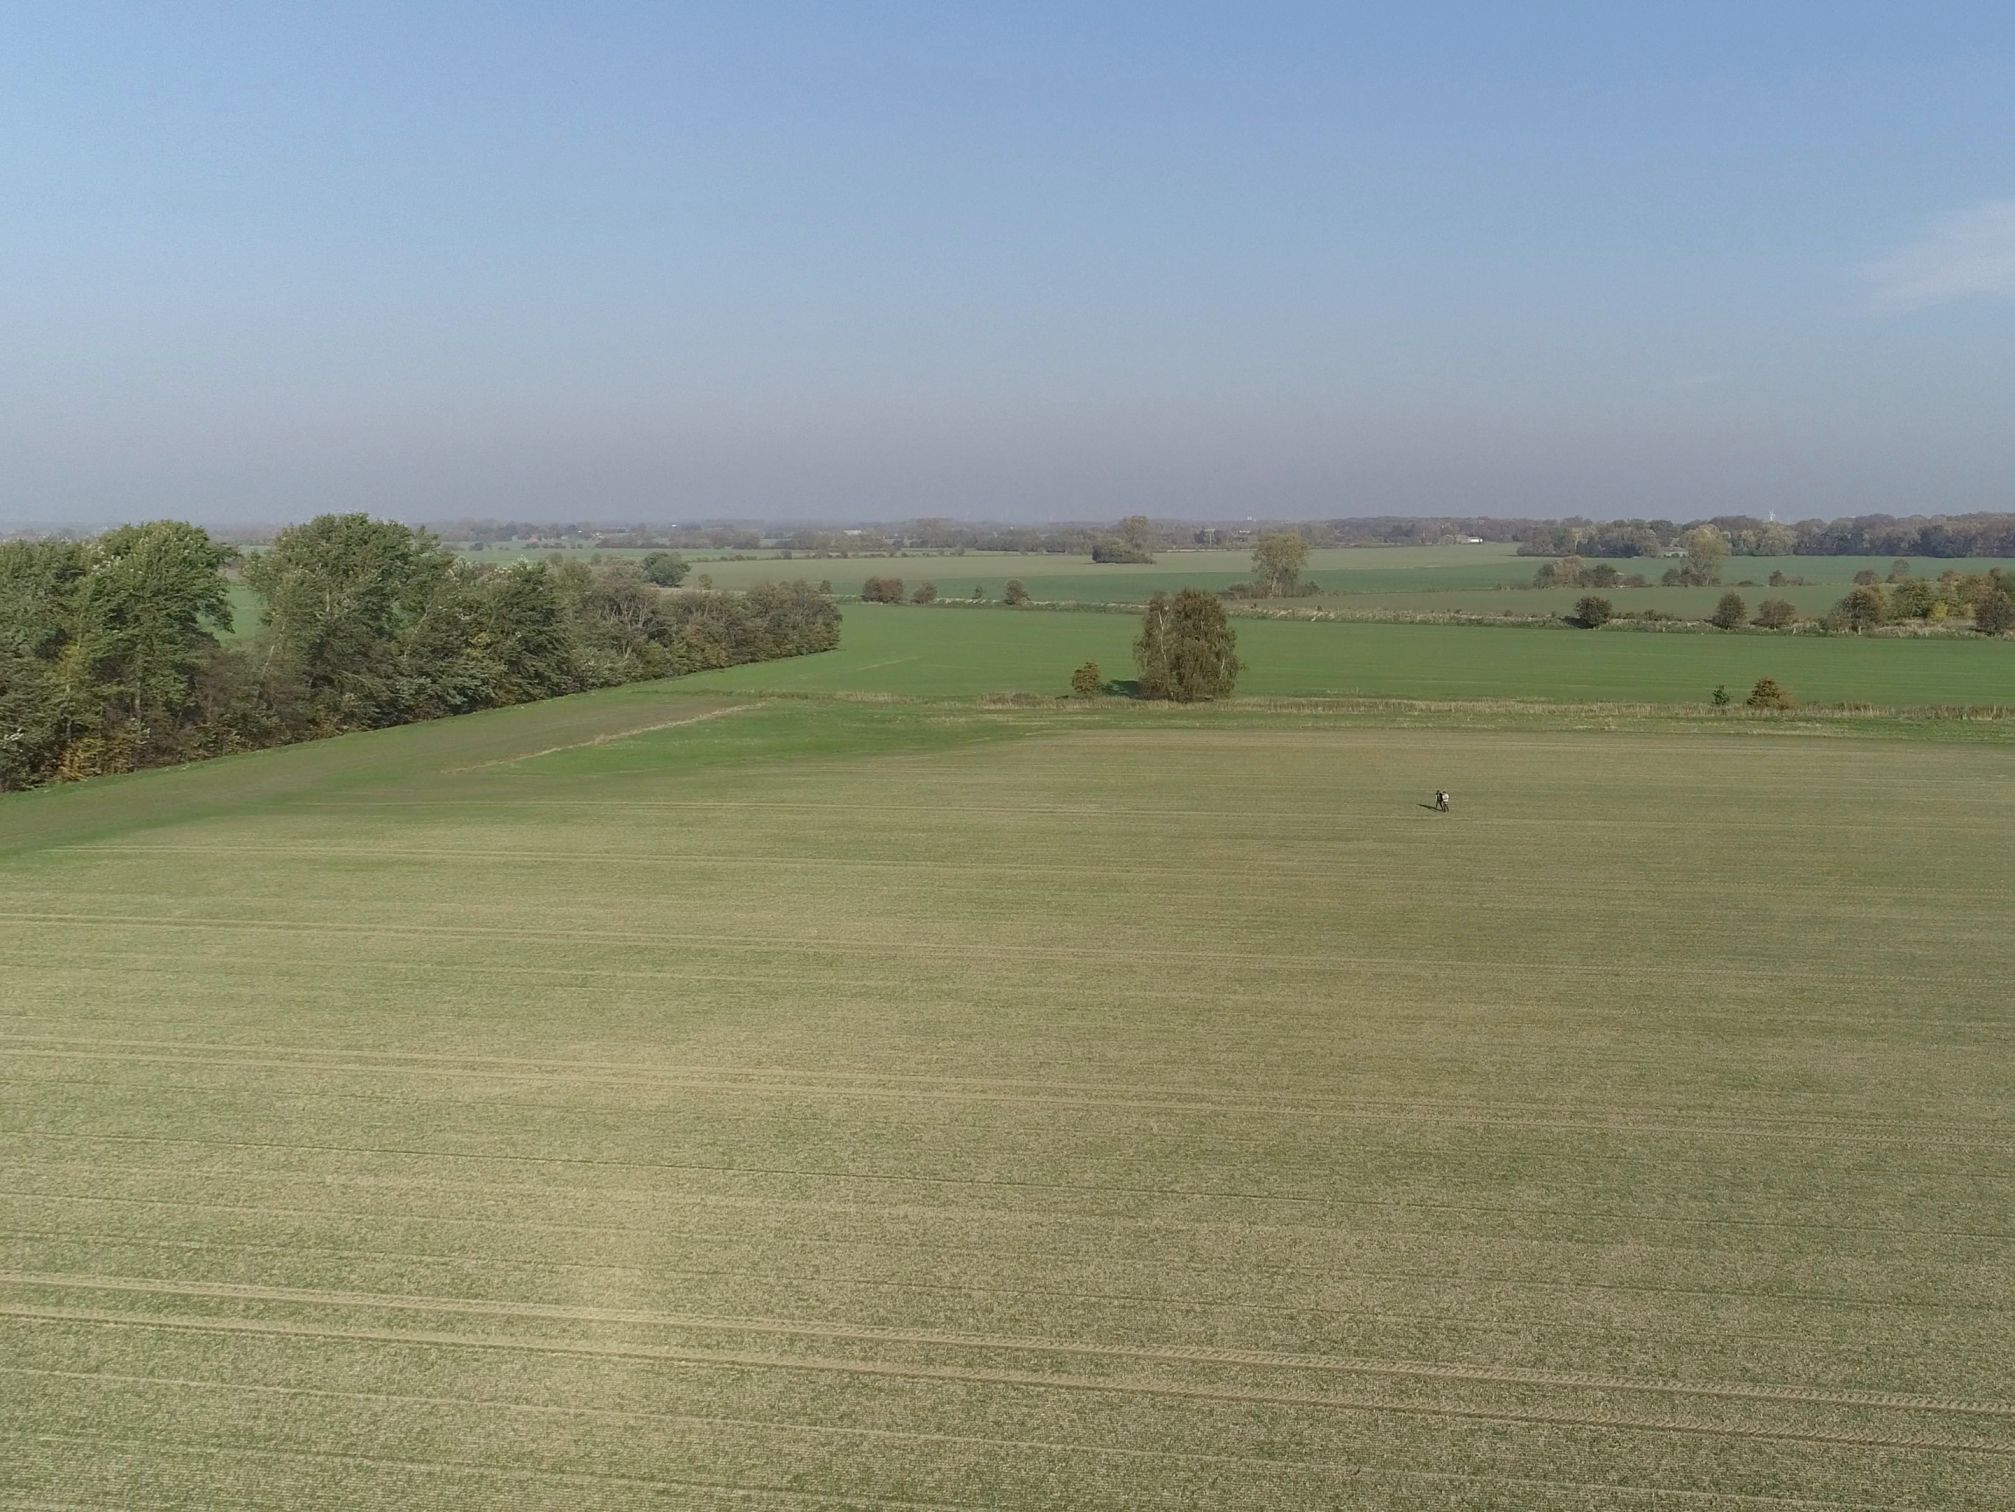
\includegraphics[width=3.122in]{figures/source/out30(1)}};

\path[fill=foo,line join=round,fill opacity=0.35,line width=0.256pt] (0.0000,247.7590) -- (227.8430,146.1690) -- (403.2000,150.1500) -- (403.2000,273.8490) -- (0.0000,247.7590) -- cycle;

\path[draw=white,line join=round,line width=0.512pt] (19.6911,244.5640) -- (56.0711,227.9040);



\path[draw=white,line join=round,line width=0.512pt] (19.8503,205.9030) -- (19.8504,244.6440) -- (67.5301,247.1570);



\path[fill=white,line join=round,line width=0.160pt] (63.6000,244.7010) -- (65.5307,247.0370) -- (63.4689,249.0560) -- (69.3046,247.0560) -- (63.6000,244.7010) -- cycle;



\path[fill=white,line join=round,line width=0.160pt] (52.5130,227.1350) -- (55.3596,228.1760) -- (54.6000,230.9590) -- (58.6260,226.2860) -- (52.5130,227.1350) -- cycle;



\path[fill=white,line join=round,line width=0.160pt] (17.6441,209.5580) -- (19.8958,207.5300) -- (22.0002,209.5030) -- (19.7535,203.7580) -- (17.6441,209.5580) -- cycle;



\path[cm={{1.0,0.0,0.0,1.0,(13.0,267.0)}}] (0.0000,0.0000) node[above right] () {\color{white}$\mathcal{O}_W$};



\path[cm={{1.0,0.0,0.0,1.0,(69.0,259.0)}}] (0.0000,0.0000) node[above right] () {\color{white}$x$};



\path[cm={{1.0,0.0,0.0,1.0,(50.0,220.0)}}] (0.0000,0.0000) node[above right] () {\color{white}$y$};



\path[cm={{1.0,0.0,0.0,1.0,(10.0,203.0)}}] (0.0000,0.0000) node[above right] () {\color{white}$z$};

\end{tikzpicture}


  \caption[The coverage problem in a precision agriculture use case]{The coverage problem in the precision agriculture use case. The aerial robot covers an agricultural field that forms a polygon (blue/transparent area in the frame), executing tasks as part of its autonomous operations {\scriptsize(photo credit: Amit Ferencz Appel)}.}
  \label{fig:plot2}
\end{figure}
We are interested in the energy optimization of the path and schedule in-flight and under uncertainty (atmospheric interferences). Such planning-scheduling finds optimal tradeoffs\findex{tradeoffs} between the path, computations, and energy requirements. Current generic solutions for, e.g., aerial robots coverage planning, do not investigate the two aspects simultaneously, nor are they energy-aware. They are often semi-autonomous. The path and computations are static and usually defined using planning software~\citep{daponte2019review} from existing algorithms~\citep{choset2001coverage,galceran2013survey}, with instances including popular flight controllers~\citep{px4,papa}. This state of practice has prompted us to investigate the possible interaction between planning-scheduling applied to coverage path planning (\Gls{acr:cpp})\findex{coverage path planning} for autonomous aerial robots. In the remainder, we will gradually build an approach that plans and schedules altogether while the aerial robot flies and its batteries drain under various conditions.

\subsection{Methodology}

Initial iterations of our work relied on case study research\findex{case study}, a widely used qualitative research\findex{qualitative research} method~\citep{darke1998successfully}. Here, we qualitatively investigated collected data and observed phenomena of the aerial robot flying early instances of the agricultural use case to derive methodologies and implications at subsequent stages. We focused on an in-depth analysis of the planning-scheduling interactions, analyzing its energy implications and the available literature. 

The grounding of further research directions involved research questions formulation: 
\begin{enumerate*}[label={(\alph*)},font={\textit}]
  \item how to model the computations energy to predict the impact of any possible schedule on the computing hardware's power? 
  \item How to model the motion energy to predict the impact of any possible variation of motion on the aerial robot's energy? 
  \item How to merge these two points with a cohesive model? 
  \item How to derive an optimal configuration of the schedule and motion?
\end{enumerate*} 

We addressed these questions using the active research\findex{active research} method cycle~\citep{gerald1978assessment}: beginning from each question, we derived a research action, deployed the action with a rigorous methodology, evaluated the results, and under unsatisfactory outcomes, adjusted the methodology. Multiple iterations of the cycle led to the energy-aware coverage planning and scheduling for autonomous robots in this work. We addressed the research question \textit{(a)} in \fref{sec:comp-ener-model}{Sections}\fref{sec:battery-model}{--\hspace*{-.8ex}}, \textit{(b)} in \fref{sec:battery-model}{Sections}\fref{sec:mot-ener-model}{--\hspace*{-.8ex}}, \textit{(c)} in \fref{sec:mot-ener-model}{Section}, and \textit{(d)} in \fref{cp:dyn}{Chapter}.


%%%%%%%%%%%%%%%%%%%%%%%%%%%%%%%%%
\section{Outline of the Approach}
\label{sec:outline}

For planning-scheduling altogether, we need some information on the intended use for both the path and computations. Path-wise, these include data on the coverage area, such as a description of an equivalent polygon. \fref{cp:pb}{Chapter} details ways of defining the problem with its building constructs (plan, stages, parameters, paths, constraints, triggering points). From the polygon, a coverage algorithm in \fref{sec:cov-path-plan}{Section} generates a plan composed of multiple stages, later eventually replanned by a replanning algorithm in case of, e.g., sudden battery drops in \fref{sec:mpc}{Section}. At each stage, the aerial robot flies a path and executes some computations. The concept of different stages serves for the purposes of modeling complex paths, e.g., multiple circles and lines form the overall coverage. The robot switches between the paths in the proximity of specific triggering points. The plan further contains some additional parameters to alter the path and computations along with an energy budget. The alterations are bounded. There are path constraint sets that bound the path alterations and computations constraint sets, one per each computation, that bound computations alterations. The approach guides the aerial robot with a vector field-based gradient descent algorithm in \fref{sec:gvf}{Section}\findex{vector field}\findex{gradient descent}. 

Computation-wise, we need an approach to specify the computations and quantify their energy contribution. \fref{cp:model}{Chapter} covers these aspects, as well as the motion and battery energy models. The approach relies on \powprof{}~\citep{powprofiler}, a tool that we introduce in \fref{sec:comp-ener-model}{Section}, part of our early studies~\citep{seewald2019component,seewald2019coarse}. The tool models the power, energy, and battery SoC of the computations, and is embedded in the future energy estimations of the aerial robot. To this end, we empirically derive and formally prove a periodic differential energy model that accounts for the uncertainty. Based on Fourier analysis, the model exploits empirical observations to include path and computations alterations. Periodicity is due to the periodic patterns in the coverage plan. Indeed, in the coverage, as well as some other autonomous scenarios, the mobile robot often iterates over a set of tasks and paths~\citep{seewald2020mechanical,seewald202Xenergy}. Given that the plan is periodic, we expect the energy consumption to evolve (approximately) periodically. \fref{cp:res}{Chapter} will back the statement with both experimental and realistic simulated findings.

Once we have a plan and all the components to model the energy and battery, in \fref{cp:dyn}{Chapter}, we can (re)plan-schedule the coverage online in-flight, aided by modern optimal control techniques, i.e., state estimation and model predictive control (MPC)~\citep{rawlings2017model,simon2006optimal}. The control is data-driven: energy sensor data estimates some coefficients of the model to predict the future energy consumption with uncertainty while obeying the energy budget--the battery capacity and other battery parameters. Our goal is to complete the plan with the highest possible parameters configuration.


%%%%%%%%%%%%%%%%%%%%%%
\section{Applications}
\label{sec:applics}

In the remainder of this work, we focus on the precision agriculture use case where we plan the coverage and schedule hazards detection. Nonetheless, the approach works with other potential use cases. Earlier collaborations between consortium members of the TeamPlay project~\citep{teamplay}, funding this work has led to a search and rescue use case, where an aerial robot detects vessels in an offshore area, eventually planning-scheduling of the search pattern and the detection rates. We briefly detailed the scenario in our earlier study~\citep{seewald2019coarse}, which has been since extended with a deadline guarantee scheduling policy~\citep{rouxel2020prego}. We have then attempted other use cases, e.g., mapping in the planetary exploration context, where we hypothesized the possibility of scheduling navigation~\citep{seewald2020beyond}. Indeed an earlier study proposes a similar technique, scheduling perception~\citep{ondruska2015scheduled}, perhaps further motivating our analysis. Simulated use cases are also possible. In an early study~\citep{zamanakos2020energy} of a use case in agricultural safety, we followed a simulated agricultural vehicle by varying the tracking algorithm. 

There are multiple possibilities to apply our approach to a broad range of real-world and simulated use cases, arising in many different fields in and outside of basic robotics research. Generally, the planning-scheduling energy awareness in this work applies to modern aerial robots with a certain degree of autonomy, whereby the robot performs at least a predefined set of tasks over a given space. Indeed most of the guidance in \fref{cp:dyn}{Chapter} works well for aerial robots, yet, one can adapt our work to other mobile robots with energy constraints. We discuss applications out of the aerial robotics domain further in \fref{cp:conc}{Chapter}. We expect the approach to be most relevant to energy-efficient mobile robots, with the best outcomes for M\&CE close to zero (the motion and computations energy contributions are similar). Such conclusion is shared with other studies researching planning-scheduling energy awareness~\citep{sudhakar2020balancing,ondruska2015scheduled,lahijanian2018resource,mei2005case,brateman2006energy}, which we discuss further in \fref{cp:soa}{Chapter}.


%%%%%%%%%%%%%%%%%%%%%%
\section{Contribution}
\label{sec:contribs}

% [!] Here I have not addressed the comment from Hector, who was suggesting to describe A an B that form the research gap. However, I think it refers more to an area where more research is needed: "[A]ny research gap you find is an area where more studies and more research need to be conducted" https://libanswers.snhu.edu/faq/264001
There are some approaches to merging planning-scheduling in different robotics use cases in the literature~\citep{mei2005case,mei2006deployment,brateman2006energy,zhang2007low,sadrpour2013experimental,sadrpour2013mission,ondruska2015scheduled,lahijanian2018resource,sudhakar2020balancing}, yet the research area remains mostly unexplored~\citep{sudhakar2020balancing,brateman2006energy}. Our work contributes with the past relevant literature to this existing research gap, proposing coverage planning and scheduling for autonomous aerial robots under stringent energy constraints. Specifically, we derive an energy model for the heterogeneous computing hardware, alongside modeling the energy contribution of the motion. We use the model in an optimal control technique similarly to past literature~\citep{zhang2007low,ondruska2015scheduled,lahijanian2018resource,brateman2006energy}, but fill the gap further with accurate energy modeling of computations and propose an actual implementation of an MPC-based algorithm. We provide a power-saving scheduling policy as opposed to simply varying the frequency of the computing hardware~\citep{zhang2007low,brateman2006energy}, and notably, our approach runs online and is dynamic, planning-scheduling in flight rather than deriving static plans-schedules~\citep{lahijanian2018resource}. It provides additional modeling rigor and incorporates battery-aware optimization as opposed to merely considering the overall energy expenditure~\citep{sudhakar2020balancing}. We vary both the path and the schedule the aerial robot flies and runs, contrary to others that vary just one of the aspects while analyzing the energy implications of the remaining~\citep{ondruska2015scheduled}.

Aside from past relevant studies, literature on topics related to computations energy modeling, battery modeling, motion planning, and aerial planning, our contribution builds from some of our past and forthcoming studies. Our computational energy modeling relies on the methodology in our early study~\citep{seewald2019coarse}, which presented the \powprof{} tool~\citep{powprofiler} for future energy predictions of heterogeneous computing hardware. We proposed an extension of \powprof{} with a component-based energy modeling approach to abstract per-component energy in a dataflow computational network in another study~\citep{seewald2019component} that we later integrated into a Robot Operating System (\Gls{acr:ros})~\citep{quigley2009ros} set-up in the following work~\citep{zamanakos2020energy}. Here we scheduled the simulated tracking of agricultural vehicles. The motion energy model we propose in \fref{cp:model}{Chapter} relies on empirical observations of the Opterra fixed-wing aerial robot flying the agricultural scenario we introduced earlier in our work~\citep{seewald2020mechanical}. We hypothesized the approach on different robots in our brief early study~\citep{seewald2020beyond}. Finally, we plan to detail the planning-scheduling energy-awareness for CPP in precision agriculture in our forthcoming study~\citep{seewald202Xenergy}, relying on all the concepts in this work. 


%%%%%%%%%%%%%%%%%%%%%%%
\section{Reading Guide}
\label{sec:structure}

In this chapter, we introduced energy-aware coverage planning and scheduling for autonomous aerial robots, the field of aerial robotics, motivated our work, and provided its objective and methodology. We then outlined the approach, proposed the applications, and discussed the contribution.

The remaining chapters have the following structure. Formal definitions of the problem and the basic constructs are subjects of \fref{cp:pb}{Chapter}. These include the plan, stages, parameters, paths, constraints, and triggering points. The chapter then contains a plan example extended in the remainder. \fref{cp:soa}{Chapter} discusses the relevant literature for computations energy and battery modeling, motion and aerial planning, and planning of computations with motion, relating each study to our approach. Planning-scheduling energy awareness requires accurate future energy predictions, and so, \fref{cp:model}{Chapter} derives computations and motion energies and battery models. It details the \powprof{} tool for computations energy modeling and the differential periodic energy and battery models. \fref{cp:dyn}{Chapter} proposes a set of algorithms for guidance, CPP, and energy-aware coverage replanning and scheduling. The guidance directs the aerial robot physically on the coverage, CPP provides a plan, covering each point in space, and energy-aware replanning replans the plan energy-wise in-flight. \fref{cp:res}{Chapter} describes the experimental setup and results. Finally, \fref{cp:conc}{Chapter} summarizes the work and concludes with the outcomes and future perspectives.

%---
%$$$

